\documentclass[border=10pt]{standalone}
\usepackage[svgnames]{xcolor}
\usepackage{amsmath}
\usepackage{pgfplots}
\pgfplotsset{compat=newest}
\usepackage[sfdefault]{FiraSans}
\usepackage{FiraMono}
\renewcommand*\familydefault{\sfdefault}
\begin{document}
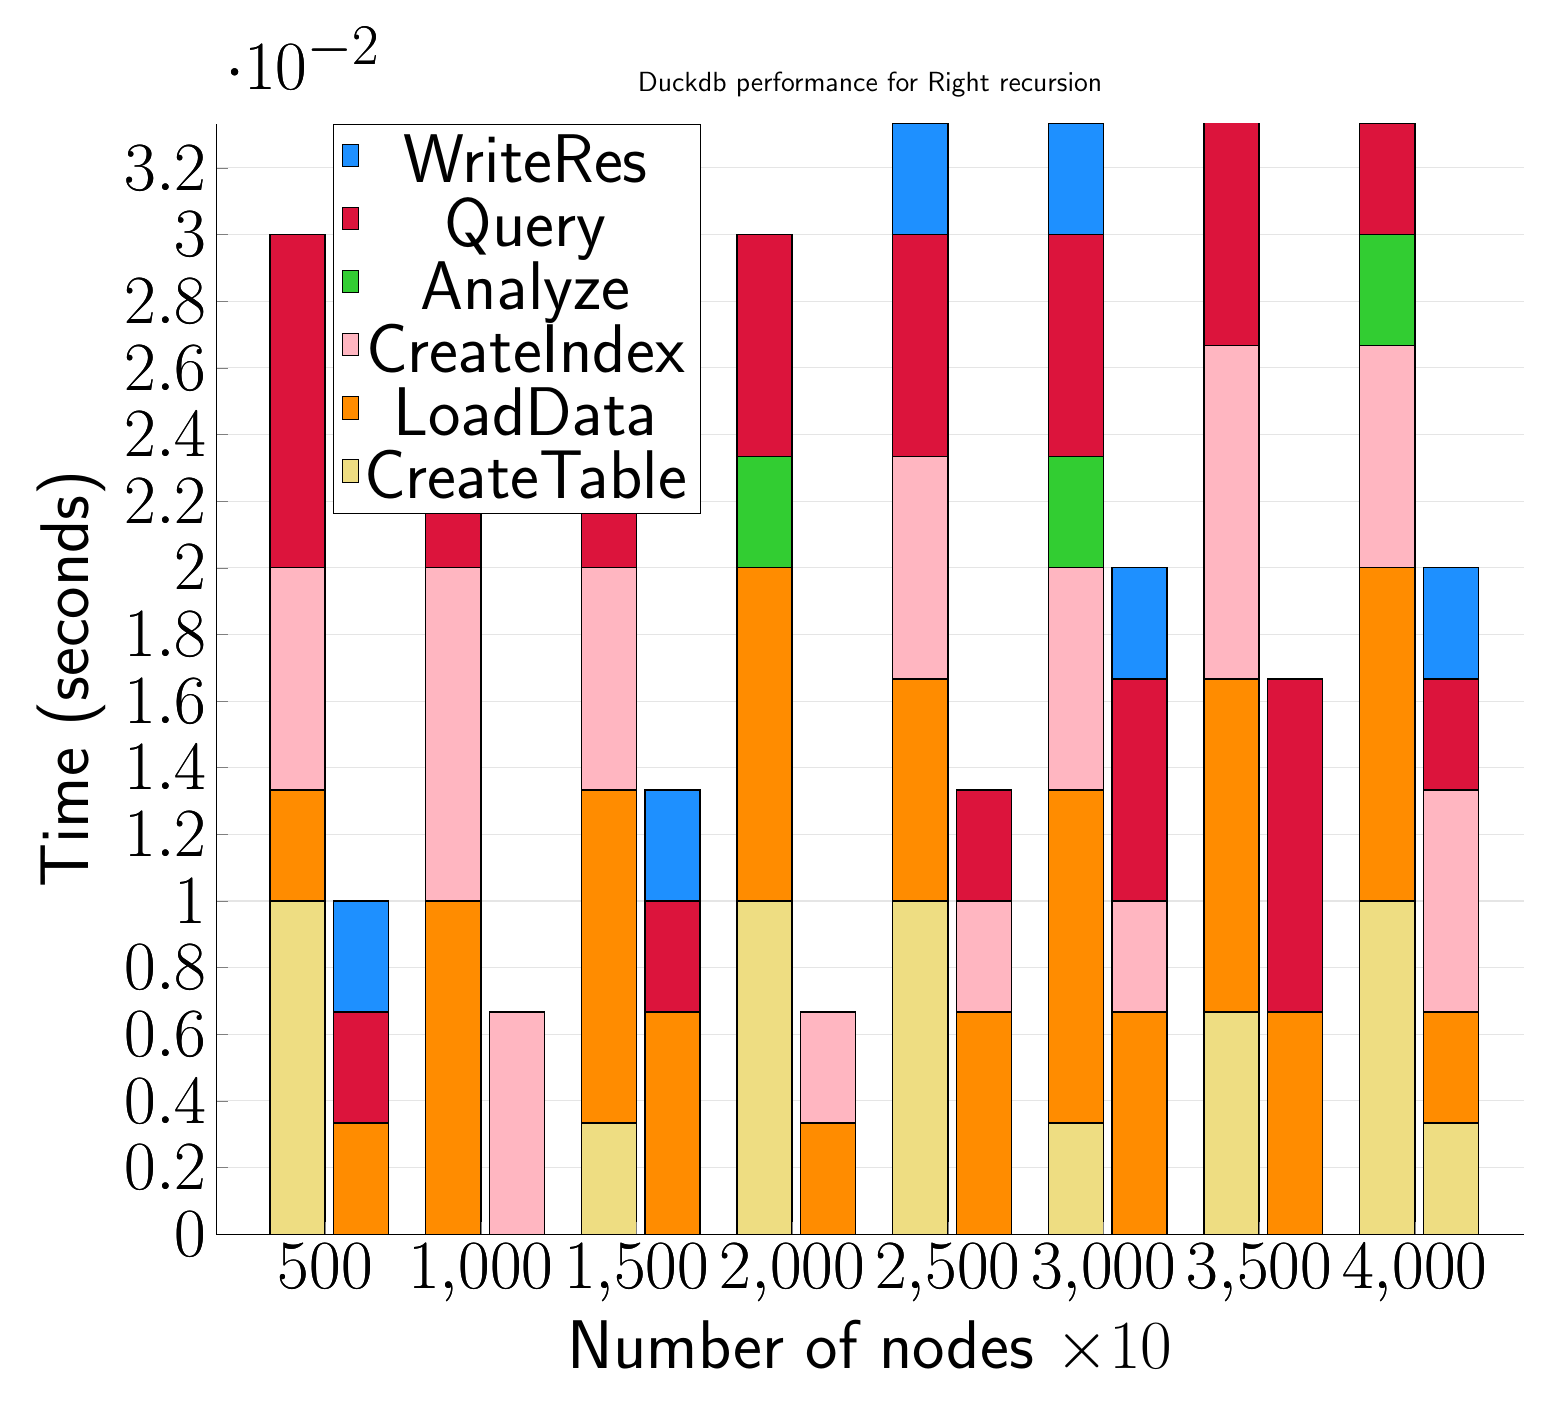
\begin{tikzpicture}
\begin{axis}[
   ybar stacked,
   title={Duckdb performance for Right recursion},
   bar shift=-10pt,
   width=1.5\textwidth,
   bar width=0.7cm,
   ymajorgrids, tick align=inside,
   major grid style={draw=gray!20},
   xtick=data,
   ymin=0, ymax=0.03333333551883698,
   axis x line*=bottom,
   axis y line*=left,
   enlarge x limits=0.1,
   legend style={
       at={(0.23, 1)},
       anchor=north,
       legend columns=1,
       font=\Huge,
   },
   ylabel={Time (seconds)},
   xlabel={Number of nodes $\times 10$},
   label style={font=\Huge},
   tick label style={font=\Huge},
]
\addlegendimage{fill=DodgerBlue, draw=black, line width=0.2pt}
\addlegendentry{WriteRes}
\addlegendimage{fill=Crimson, draw=black, line width=0.2pt}
\addlegendentry{Query}
\addlegendimage{fill=LimeGreen, draw=black, line width=0.2pt}
\addlegendentry{Analyze}
\addlegendimage{fill=LightPink, draw=black, line width=0.2pt}
\addlegendentry{CreateIndex}
\addlegendimage{fill=DarkOrange, draw=black, line width=0.2pt}
\addlegendentry{LoadData}
\addlegendimage{fill=LightGoldenrod, draw=black, line width=0.2pt}
\addlegendentry{CreateTable}
\addplot +[fill=LightGoldenrod, draw=black, line width=0.5pt] coordinates {
    (500, 0.010000000397364298)
    (1000, 0.0)
    (1500, 0.0033333351214726767)
    (2000, 0.010000000397364298)
    (2500, 0.010000000397364298)
    (3000, 0.0033333351214726767)
    (3500, 0.006666665275891622)
    (4000, 0.009999997913837433)
};
\addplot +[fill=DarkOrange, draw=black, line width=0.5pt] coordinates {
    (500, 0.003333332637945811)
    (1000, 0.010000002880891165)
    (1500, 0.010000000397364298)
    (2000, 0.009999997913837433)
    (2500, 0.0066666677594184875)
    (3000, 0.009999997913837433)
    (3500, 0.010000000397364298)
    (4000, 0.009999997913837433)
};
\addplot +[fill=LightPink, draw=black, line width=0.5pt] coordinates {
    (500, 0.0066666677594184875)
    (1000, 0.009999997913837433)
    (1500, 0.0066666677594184875)
    (2000, 0.0)
    (2500, 0.0066666677594184875)
    (3000, 0.006666665275891622)
    (3500, 0.010000002880891165)
    (4000, 0.0066666677594184875)
};
\addplot +[fill=LimeGreen, draw=black, line width=0.5pt] coordinates {
    (500, 0.0)
    (1000, 0.0)
    (1500, 0.0)
    (2000, 0.0033333351214726767)
    (2500, 0.0)
    (3000, 0.003333332637945811)
    (3500, 0.0)
    (4000, 0.0033333351214726767)
};
\addplot +[fill=Crimson, draw=black, line width=0.5pt] coordinates {
    (500, 0.010000000397364298)
    (1000, 0.009999997913837433)
    (1500, 0.009999997913837433)
    (2000, 0.0066666677594184875)
    (2500, 0.006666665275891622)
    (3000, 0.0066666702429453535)
    (3500, 0.009999997913837433)
    (4000, 0.003333332637945811)
};
\addplot +[fill=DodgerBlue, draw=black, line width=0.5pt] coordinates {
    (500, 0.0)
    (1000, 0.0)
    (1500, 0.0)
    (2000, 0.0)
    (2500, 0.003333332637945811)
    (3000, 0.003333332637945811)
    (3500, 0.0)
    (4000, 0.0066666677594184875)
};
\end{axis}
\begin{axis}[
   ybar stacked,
   bar shift=13pt,
   width=1.5\textwidth,
   bar width=0.7cm,
   ymajorgrids, tick align=inside,
   major grid style={draw=none},
   xtick=data,
   ymin=0, ymax=0.03333333551883698,
   axis x line*=none,
   axis y line*=none,
   enlarge x limits=0.1,
   label style={font=\Huge},
   tick label style={font=\Huge},
]
\addplot +[fill=LightGoldenrod, draw=black, line width=0.5pt] coordinates {
    (500, 0.0)
    (1000, 0.0)
    (1500, 0.0)
    (2000, 0.0)
    (2500, 0.0)
    (3000, 0.0)
    (3500, 0.0)
    (4000, 0.003333333333333318)
};
\addplot +[fill=DarkOrange, draw=black, line width=0.5pt] coordinates {
    (500, 0.003333333333333336)
    (1000, 0.0)
    (1500, 0.006666666666666672)
    (2000, 0.003333333333333336)
    (2500, 0.006666666666666672)
    (3000, 0.006666666666666668)
    (3500, 0.006666666666666672)
    (4000, 0.003333333333333336)
};
\addplot +[fill=LightPink, draw=black, line width=0.5pt] coordinates {
    (500, 0.0)
    (1000, 0.006666666666666672)
    (1500, 0.0)
    (2000, 0.003333333333333337)
    (2500, 0.003333333333333336)
    (3000, 0.003333333333333336)
    (3500, 0.0)
    (4000, 0.006666666666666654)
};
\addplot +[fill=LimeGreen, draw=black, line width=0.5pt] coordinates {
    (500, 0.0)
    (1000, 0.0)
    (1500, 0.0)
    (2000, 0.0)
    (2500, 0.0)
    (3000, 0.0)
    (3500, 0.0)
    (4000, 0.0)
};
\addplot +[fill=Crimson, draw=black, line width=0.5pt] coordinates {
    (500, 0.003333333333333336)
    (1000, 0.0)
    (1500, 0.0033333333333333184)
    (2000, 0.0)
    (2500, 0.0033333333333333184)
    (3000, 0.006666666666666654)
    (3500, 0.009999999999999986)
    (4000, 0.003333333333333336)
};
\addplot +[fill=DodgerBlue, draw=black, line width=0.5pt] coordinates {
    (500, 0.003333333333333318)
    (1000, 0.0)
    (1500, 0.003333333333333336)
    (2000, 0.0)
    (2500, 0.0)
    (3000, 0.0033333333333333184)
    (3500, 0.0)
    (4000, 0.003333333333333336)
};
\end{axis}
\end{tikzpicture}

\end{document}
